% Paper for CCGrid 2027, Track 5 (Performance Modeling, Analysis, and Optimization).
% Limit: 10 IEEE pages including references; double-blind review (no names, no repository links).
% Build: make (latexmk -pdf). \todo{} marks what is still missing.
\documentclass[conference]{IEEEtran}
\usepackage[utf8]{inputenc}
\usepackage[T1]{fontenc}
\usepackage{cite}
\usepackage{amsmath,amssymb}
\usepackage{graphicx}
\usepackage{booktabs}
\usepackage{xcolor}
\usepackage{url}
\usepackage[hidelinks]{hyperref}
\usepackage{cleveref}
% For the final submission: switch to \usepackage[disable]{todonotes}
\usepackage[colorinlistoftodos,textsize=tiny]{todonotes}
\newcommand{\anonrepo}{\url{https://anonymous.4open.science/r/XXXX}\todo{anonymous artifact link}}
\graphicspath{{figs/}}

\begin{document}

\title{Sidecars, Ambient, or eBPF? Measuring the Tail-Latency and Resource Cost of Kubernetes Service Meshes}

% Double-blind: no names, affiliations, or e-mails
\author{\IEEEauthorblockN{Anonymous Author(s)}
\IEEEauthorblockA{Anonymous Institution}}

\maketitle

\begin{abstract}
Service meshes add mutual TLS, telemetry, and traffic policy to microservices, but each data-plane design pays for
them differently: a proxy per pod (sidecar), a per-node L4 proxy with optional shared L7 waypoints (ambient), or
in-kernel eBPF with a per-node proxy. We measure six configurations---no mesh, Istio sidecar, Istio ambient with and
without waypoints, Linkerd, and Cilium with WireGuard and L7 policy---on a pinned, virtualized Kubernetes testbed with
open-loop load at 30, 60, and 90\% of the lowest saturation throughput among the configurations, using a synthetic echo service, Online Boutique,
and DeathStarBench Hotel Reservation. On Online Boutique at 60\% load, the Istio sidecar adds 52\,ms to p99 latency, while
ambient L4 adds 6.7\,ms; per 1000~req/s the extra CPU ranges from 2.6 (ambient L4) to 7.0 (Cilium) cores, and
energy per request grows by 16 to 188\% at 90\% load. Profiling attributes most of the overhead to HTTP/2 processing for the Istio sidecar (61\% of its data-plane
CPU), TLS for ambient L4 (47\%), and the per-node Envoy, agent, and WireGuard for Cilium. A compositional model built from per-hop proxy cost and a queueing term, fitted on two
applications, predicts the third application's p99 overhead within 11\% for ambient L4, but not for L7 data planes, whose tail is set by the busiest node. We distill the results into
a decision guide for choosing a data plane.
\end{abstract}

\begin{IEEEkeywords}
service mesh, Kubernetes, tail latency, performance evaluation, eBPF, energy efficiency
\end{IEEEkeywords}

% ---------------------------------------------------------------------------------------------------------------
% 01-introduction.tex
\section{Introduction}
\label{sec:intro}

Service meshes have become the default way to add mutual TLS, fine-grained
traffic policy, and request-level telemetry to microservices on Kubernetes,
without changing application code. The price is paid on every request: traffic
that used to flow directly between two pods now crosses one or more proxies,
each of which terminates connections, encrypts and decrypts traffic, and often
parses application-layer protocols. In deep call graphs, this cost is paid at
every hop, and it shows up where operators care most: in the tail of the
latency distribution and in the CPU that must be provisioned for it.

The design space of service meshes has changed considerably in the last few
years. The original \emph{sidecar} architecture, in which a proxy runs next to
every application container (Istio with Envoy, Linkerd with its Rust
\texttt{linkerd2-proxy}), now competes with \emph{sidecar-less} designs. Istio
Ambient splits the data plane into a per-node L4 proxy (ztunnel) and optional,
shared L7 proxies (waypoints), while Cilium implements L3/L4 functions in eBPF
inside the kernel and delegates L7 processing to a per-node Envoy. Each design
moves work to a different place (the pod, the node, or the kernel) and changes
how many proxies a request traverses, so their costs cannot be inferred from
one another.

The most detailed study of mesh overheads to date, MeshInsight~\cite{zhu2023meshinsight},
decomposed the cost of the Istio sidecar into its components and found that it
can raise latency by up to 269\% and CPU usage by up to 163\%. That analysis,
however, covers only the Envoy sidecar, profiles it with at most one
outstanding request, and its model explicitly cannot predict tail latency. More recent comparisons of sidecar and
sidecar-less meshes~\cite{bremlerbarr2024mtls} examine mTLS alone, on a
synthetic server with an artificial delay, without L7 processing, waypoints,
energy, or a predictive model. Operators choosing a mesh today therefore lack a
same-testbed comparison of the architectures they can actually deploy.

This paper provides that comparison. We measure seven configurations on the same
testbed: no mesh, Istio sidecar, Istio Ambient with and without a waypoint,
Linkerd, and Cilium service mesh with and without L7 policy, each with east-west encryption enabled
in its default data path: workload-level mutual TLS for Istio and Linkerd,
and node-to-node WireGuard for Cilium. We drive an echo
microbenchmark and two widely used microservice benchmarks, Online
Boutique~\cite{onlineboutique} and Hotel Reservation from
DeathStarBench~\cite{gan2019deathstarbench}, with open-loop load, which avoids
the coordinated-omission bias that hides tail latency~\cite{tene2015latency}.
Our contributions are:

\begin{itemize}
  \item \textbf{A same-testbed measurement of seven mesh configurations}
        (RQ1). We report p99 and p99.9 latency, maximum SLO-compliant
        throughput, CPU, memory, and energy per request, with ten randomized
        repetitions per cell for latency and resources (five for Cilium
        without L7 policy), three for energy, and
        non-parametric statistics. Sidecar-based
        Istio sustains only 30\% of the no-mesh throughput on the echo
        benchmark, while ambient L4 mode retains 78\%.
  \item \textbf{An attribution of overhead beyond Envoy} (RQ2). Using perf and
        eBPF, we break the cost down into TLS, L7 parsing, socket I/O, context
        switches, and kernel time, including ztunnel, the Ambient waypoint,
        \texttt{linkerd2-proxy}, and Cilium's agent, per-node Envoy, and
        WireGuard. Ablations show that Cilium's cost comes from the L7
        redirect and Hubble flow logging, not from its eBPF programs.
  \item \textbf{A model of the tail and its limits} (RQ3). A compositional
        model of per-hop proxy cost, cross-node hops, and queueing, fitted on
        two applications, explains the p99 of the third within 11--13\% for
        the L4 data planes; for per-pod sidecars, queueing at the busiest
        proxy instance cuts the error from 82\% to 19\% (Linkerd) and from
        135\% to 52\% (Istio), while node utilization does not explain it.
        Node utilization bounds throughput within 19\% on the two
        microservice applications. A placement experiment shows that node
        load explains the tail of L7 data planes only partly.
  \item \textbf{A decision guide} (RQ4) that maps latency, CPU, and energy
        budgets to the mesh that satisfies them.
\end{itemize}

We also partially reproduce MeshInsight: the CPU overhead of the Istio
sidecar on Online Boutique falls within the published range, but its latency
overhead is larger (\cref{sec:validation}). We release the testbed, scripts, and data to
support reproduction at \anonrepo.

The rest of the paper is organized as follows. \Cref{sec:background} describes
the mesh architectures we compare, \cref{sec:related} discusses related work,
\cref{sec:method} presents the testbed and methodology, and
\cref{sec:rq1,sec:rq2,sec:rq3,sec:rq4} answer the four research questions.
\Cref{sec:threats} discusses threats to validity and \cref{sec:conclusion}
concludes.

% 02-background.tex
\section{Background: Service Mesh Data Planes}
\label{sec:background}

A service mesh has a \emph{control plane}, which distributes identities,
certificates, and routing policy, and a \emph{data plane}, which handles
application traffic. Our measurements concern the data plane, whose
architecture determines how many proxies a request crosses and where their work
is executed. \Cref{tab:configs} summarizes the configurations we study.

\paragraph{Per-pod sidecars}
In Istio's sidecar mode, an Envoy proxy is injected into every pod, and
iptables rules redirect all inbound and outbound traffic through it. A request
between two services therefore traverses two proxies, each of which terminates
TCP, performs mTLS, and parses HTTP or gRPC to apply L7 policy and collect
telemetry. Linkerd uses the same pattern with \texttt{linkerd2-proxy}, a
purpose-built proxy written in Rust that implements a smaller feature set.

\paragraph{Istio Ambient}
Ambient mode removes the sidecar. A per-node proxy, ztunnel, captures pod
traffic and carries it between nodes over mTLS in an HTTP CONNECT-based tunnel
(HBONE). ztunnel provides L4 functions only: identity, encryption, and L4
authorization. When L7 features are required, traffic is additionally routed
through a \emph{waypoint}, a shared Envoy deployment that serves a namespace or
a service account. Ambient therefore has two operating points, L4-only (IA4)
and L4 plus waypoint (IA7), which we measure separately.

\paragraph{Cilium service mesh}
Cilium implements networking, load balancing, and L3/L4 policy with eBPF
programs attached to the kernel datapath. Transparent encryption between nodes
uses WireGuard (or IPsec), and L7 policy is enforced by redirecting the matching
traffic to an Envoy instance shared by all pods on the node. Unlike the other
meshes, Cilium encrypts at the node level rather than per workload, and only
traffic subject to an L7 rule is sent through a proxy. We measure Cilium both with an L7
rule on every application port (CI) and without one (CI4).

We compare each mesh's default data path for east-west encryption, not equal
functionality: the configurations differ in what they authenticate, whether
same-node traffic is encrypted, and how much L7 telemetry they produce
(\cref{tab:configs}).

\paragraph{Where the cost goes}
These designs differ in three ways that matter for performance: the number of
user-space proxies on the request path (two for sidecars, zero to two for
Ambient and Cilium), whether those proxies are dedicated to a pod or shared by
a node, and how much work is moved into the kernel. Shared proxies amortize
memory but concentrate CPU on the node that hosts them, which, as we show in
\cref{sec:rq1}, matters for tail latency under load.

\begin{table}[t]
  \centering
  \caption{Configurations measured, each in its default data path. mTLS:
           workload identity and mutual TLS; same-node: encryption of calls
           between pods on the same node; L7: where HTTP/gRPC is processed;
           telemetry: L7 telemetry produced by default.}
  \label{tab:configs}
  \footnotesize
  \setlength{\tabcolsep}{2pt}
  \begin{tabular}{@{}llcccl@{}}
    \toprule
    ID  & Data plane             & mTLS & Same-node & L7 & Telemetry \\
    \midrule
    B   & none (Cilium CNI)  & --   & --  & --          & -- \\
    IS  & Envoy per pod      & yes  & yes & per pod   & Envoy \\
    IA4 & ztunnel per node   & yes  & yes & --          & L4 only \\
    IA7 & ztunnel + waypoint & yes & yes & waypoint & Envoy \\
    LK  & Rust proxy per pod & yes & yes & per pod & proxy \\
    CI  & eBPF, WG, Envoy per node & no$^{\dagger}$ & no & node & Hubble (L7) \\
    CI4 & eBPF, WG                 & no$^{\dagger}$ & no & --   & Hubble (L4) \\
    \bottomrule
    \multicolumn{6}{@{}p{0.95\columnwidth}@{}}{\scriptsize $^{\dagger}$Nodes, not workloads, are
    authenticated (WireGuard, WG); Cilium's mutual authentication is not enabled.}
  \end{tabular}
\end{table}

% 03-related.tex
\section{Related Work}
\label{sec:related}

\paragraph{Component-level analysis of sidecars}
MeshInsight~\cite{zhu2023meshinsight} is the work closest in method to ours.
It profiles the Istio sidecar (Istio 1.13, Envoy 1.21) on Online Boutique and
Hotel Reservation and attributes its overhead to seven components, finding that
protocol parsing dominates. It reports latency increases of 27--269\% and CPU
increases of 42--163\%, depending on configuration, and proposes a linear
compositional model of overhead. The authors note that the model does not
predict tail latency, and that extending the analysis to other meshes is future
work. We extend the analysis to ztunnel, the Ambient waypoint,
\texttt{linkerd2-proxy}, and Cilium's eBPF datapath, use open-loop load, add
energy, and model the tail through a queueing term.

\paragraph{Comparisons of sidecar and sidecar-less meshes}
Bremler-Barr et al.~\cite{bremlerbarr2024mtls} compare Istio sidecar, Istio
Ambient (ztunnel only), Linkerd, and Cilium, focusing on the cost of mTLS. Their
workload is a synthetic server with a fixed 200\,ms delay driven by Fortio, and
they do not exercise L7 processing, waypoints, or realistic call graphs. They
also observe that Cilium does not encrypt traffic between pods on the same node,
a caveat that applies to our setup as well: under our placement, 2.8 of the
3.8 internal calls per Hotel Reservation request, and 0.6 of the 11 per Online
Boutique request, stay on one node and are therefore not encrypted by Cilium's
WireGuard. Our study uses multi-service
applications, includes the waypoint, and reports energy and a predictive model.

\paragraph{Reducing mesh overhead}
A separate line of work proposes new data-plane designs rather than measuring
existing ones. Meshlib~\cite{mostafaei2026meshlib} builds on Cilium and enforces
L7 policy inside the application process through an optional library, falling
back to Cilium's per-node Envoy for unmodified services; on TrainTicket, a
single node and up to 200\,req/s, it reports lower latency than Istio, Linkerd,
and unmodified Cilium, and attributes most of the cost of L7 proxying to
protocol parsing. Cvetkovi\'c and Klimovic~\cite{cvetkovic2025lightweight}
characterize Istio and Linkerd sidecars on Knative and report 38.3$\times$
higher p95 execution time with Istio policies and up to 3.9$\times$ higher p95
CPU per worker; they could not evaluate Ambient, which Knative does not
support. Neither evaluates Istio Ambient or energy. Our measurements are complementary: they quantify the cost these
designs aim to remove, on the architectures in production today.

\paragraph{Microservice benchmarks and load generation}
We use Online Boutique~\cite{onlineboutique} and Hotel Reservation from
DeathStarBench~\cite{gan2019deathstarbench}, the same applications as
MeshInsight, so that results can be compared directly. We generate open-loop
load with k6~\cite{k6} at a constant arrival rate, avoiding the
coordinated-omission problem of closed-loop generators, which underestimates
tail latency~\cite{tene2015latency}. Energy is measured with Intel
RAPL~\cite{khan2018rapl}.
Container-level energy estimators for Kubernetes such as Kepler have been
found inaccurate~\cite{pijnacker2025kepler}, and per-task RAPL attribution on
shared nodes must fall back to approximations from CPU
utilization~\cite{thamm2025rapl}; we therefore report package-level energy per
request for the whole host rather than per container.

% 04-methodology.tex -- versions as recorded by the testbed scripts at run time.
\section{Testbed and Methodology}
\label{sec:method}

\subsection{Testbed}
\label{sec:testbed}

All experiments run on a single dedicated host with an Intel Core i7-12700K
(8 performance cores with two hardware threads each, plus 4 efficiency cores)
and 64\,GB of RAM. To reduce measurement noise, we set the frequency governor
to \texttt{performance}, disable turbo boost, and disable idle states deeper
than C1, following MeshInsight~\cite{zhu2023meshinsight}.

The cluster runs in four KVM virtual machines (Ubuntu 24.04, kernel
6.8.0-149) managed with libvirt. Every vCPU is pinned to a dedicated
physical thread of a performance core: the control-plane VM has 2 vCPUs and
6\,GB, and each of the three worker VMs has 4 vCPUs and 14\,GB. QEMU emulator
threads are pinned to a separate core pair, so no two VMs share a physical
core. Kubernetes is k3s v1.37.2, with Cilium 1.20.3 as the CNI in
every configuration, so that the baseline and the meshes share the same
underlying network. We install Istio 1.32.0, Linkerd
edge-26.11.1, and Cilium's service-mesh features from their upstream
releases with default proxy settings; all versions are pinned in the
artifact.

\paragraph{Mesh configuration}
Every mesh encrypts east-west traffic in its default data path
(\cref{tab:configs}). For Istio (IS, IA4, IA7) we apply a mesh-wide
\texttt{STRICT} \texttt{PeerAuthentication}, and for Linkerd a default policy
that only admits authenticated mesh traffic, so both require workload-level
mutual TLS. For Cilium we enable WireGuard encryption between nodes and a
\texttt{CiliumNetworkPolicy} with L7 HTTP rules on the application ports,
which activates the per-node Envoy; Cilium's workload-level mutual
authentication is not enabled, so it authenticates nodes, not workloads, and
does not encrypt same-node traffic. In IA7, each application namespace has its
own waypoint. Only the entry service of each application accepts plaintext
traffic from the load generator.

\paragraph{Cilium settings}
The same Cilium installation serves as the CNI in all six configurations. It
runs with kube-proxy replacement enabled, so service load balancing is done by
eBPF programs at each pod's network interface, but with socket-level load
balancing limited to the host namespace, a setting that Istio and Linkerd
require to see the original service address; pod traffic is carried between
nodes in a VXLAN tunnel. Hubble, Cilium's flow observability, is on by
default, and in CI the per-node Envoy sends its L7 access logs to it.

\paragraph{Placement}
Control-plane components (istiod, the Linkerd control plane, the Cilium
operator, CoreDNS, and Prometheus) run on the control-plane VM, so they do not
compete with the data plane. Application pods are assigned to the three workers
round-robin with a fixed order, so every configuration uses the same placement,
and each waypoint is pinned to a fixed worker. We remove the demonstration CPU
and memory limits and the liveness probes shipped with the benchmark manifests,
keeping requests and readiness probes: in a pilot, those limits throttled
individual services and caused restarts that would have dominated the
results. Mesh proxies keep their default resource settings. The busiest sidecar, the
frontend's in IS on OB at 90\% load, used a median of 1.28 cores per run
(peak 1.36 in a 5\,s sample), below its default limit of 2 CPUs and 2 worker
threads.

\paragraph{Applications}
We use three workloads. \emph{Echo} is a two-service chain of Fortio
servers (a relay forwarding each request to an echo server on another worker),
which isolates the per-hop cost of the data plane. \emph{Online Boutique}
(OB)~\cite{onlineboutique} has 11 services communicating over gRPC, with its
built-in load generator removed. \emph{Hotel Reservation}
(HR)~\cite{gan2019deathstarbench} has eight Go services that communicate over
gRPC, a Consul registry, and six MongoDB and three memcached instances. The k6 scripts emulate user sessions: for OB, browsing the home
page, viewing products, changing currency, and adding to the cart; for HR, 60\%
hotel search, 39\% recommendations, 0.5\% logins, and 0.5\% reservations.

\paragraph{Reproducible state}
Each configuration is deployed from the same base snapshot of all four VMs,
which contains the cluster and every container image already pulled, so no run
downloads images and every configuration starts from an identical state.
Automatic package updates are disabled inside the VMs.

\subsection{Load generation}
\label{sec:load}

The load generator, k6~\cite{k6}, runs on the host, pinned to the four
efficiency cores, which no VM uses. It issues requests at a constant arrival
rate (open loop), so a slow response does not delay subsequent requests and
tail latency is not hidden~\cite{tene2015latency}. At the highest rates we
used, the generator's cores were about 53\% utilized, and we track dropped
iterations to detect client saturation.

\paragraph{Saturation}
For each configuration and application, we first estimated the maximum
SLO-compliant throughput before the main experiment, by increasing the rate in
steps of 25\%, each held for 60\,s, until p99 latency exceeded the SLO
(20\,ms for echo, 500\,ms for OB, 100\,ms for HR) or more than 1\% of
requests failed or were dropped; the last passing rate was confirmed with one
more step. After the main experiment, we refined each boundary with four
bisection steps between the last passing and the first failing rate of that
search (a resolution of about 1.5\% of the rate). \Cref{tab:sat} reports the
highest tested rate that met the SLO; in 12 of the 18 cells every bisection
step passed, so the next tested rate is the one that failed once in the
initial search. Saturation is a single search per configuration and
application, without repetitions.

\paragraph{Load levels}
All configurations must be compared at the same absolute request rate, and a
rate beyond a mesh's saturation would measure queue collapse rather than
overhead. We therefore set three load levels per application at 30\%, 60\%,
and 90\% of the \emph{lowest} initial saturation estimate among the six
configurations (2382\,req/s for echo, 643 for OB, and 865 for HR). This yields
714, 1429, and 2143\,req/s for echo, 192, 385, and 578\,req/s for OB, and 259,
519, and 778\,req/s for HR. Throughout the paper, ``30/60/90\% load'' refers to
these fixed rates. Measured against the refined lowest saturation
(\cref{tab:sat}: 2939, 793, and 1067\,req/s), they correspond to about 24\%,
49\%, and 73\% for all three applications, so even the highest level leaves
every configuration some headroom.

\subsection{Experiment design and metrics}
\label{sec:design}

The main experiment crosses 6 configurations, 3 applications, and 3 load
levels, with 10 repetitions per cell, for 540 runs. Latency and resource
metrics come from these 10 repetitions; energy comes from 3 repetitions per
cell of a second run (below); saturation is a single search. Within each configuration,
the order of runs is randomized with a fixed seed. Each run has 60\,s of
warm-up, which is discarded, followed by 180\,s of measurement.

We collect: (i) latency percentiles (p50, p90, p99, p99.9), error rate, and
achieved throughput from k6; (ii) CPU and memory per container (application,
sidecar, ztunnel, waypoint, Cilium agent and Envoy, control plane) from
cAdvisor through Prometheus at a 5\,s interval; and (iii) package and core
energy from RAPL on the host. We subtract the idle power of the no-mesh
baseline from every configuration, so that each mesh's standing cost is
included, and report joules per request together with each mesh's idle power
above the baseline. Energy comes from a second run of the same cells (30\%
and 90\% load, 3 repetitions) with KVM halt-polling disabled
(\cref{sec:threats}); latency and resource results come from the main run.
Without halt-polling, p99 stayed within 10\% of the main run in 25 of the 36
cells; the baseline itself became 10--29\% faster, and the largest mesh changes
were Ambient L4 on echo (+15 to +29\%) and the waypoint on HR at 90\% load
($-$24\%), so overheads relative to the baseline are, if anything, conservative
in the main run for most meshes. Resource
costs are also
normalized to millicores and MiB per 1{,}000\,req/s.

For profiling (RQ2), we repeat each configuration at the 60\% load level and
record call stacks with \texttt{perf} on the worker VMs and count context
switches and system calls per request with eBPF (bpftrace).

\paragraph{Statistics}
We report medians across repetitions with 95\% bootstrap confidence intervals.
We test for differences among configurations with the Kruskal--Wallis test and
compare each mesh with the baseline using the Mann--Whitney U test with Holm
correction, reporting Cliff's $\delta$ as the effect size. The coefficient of
variation of p99 across repetitions measures the predictability of each mesh.

\subsection{Partial Reproduction of MeshInsight}
\label{sec:validation}

To check how far a single-host testbed reproduces published behavior, we repeated
MeshInsight's comparison of the Istio sidecar against no mesh on Online
Boutique, with five repetitions per configuration. At 275\,req/s, the sidecar
increased cluster CPU usage by 129\%, within the published range of
42--163\%~\cite{zhu2023meshinsight}. Latency increased by 416\% (p50) and 440\%
(p99), above the published 27--269\%, so the reproduction is partial: CPU
reproduces, latency does not. At 551\,req/s the latency increase grew
further (p50 +1482\%), while CPU rose by 80\%. We attribute the higher latency
to two factors that we analyze in \cref{sec:rq1,sec:rq3}: a newer Istio and
Envoy, and the concentration of sidecar work on the node that hosts the
frontend, which reached 77\% utilization at 551\,req/s. The main experiment shows
the same effect: for the Istio sidecar on OB at 90\% load, the busiest worker
is 76\% utilized, against 43\% without a mesh.

% 05-results.tex -- results of the main run (540 runs, 17/11) and of the energy run
% with KVM halt-polling disabled (108 runs, 18/11). Numbers are medians across
% repetitions; tables are generated by analysis/*.py.

\section{RQ1: What Does Each Mesh Cost?}
\label{sec:rq1}

\paragraph{Throughput}
\Cref{tab:sat} reports the maximum throughput each configuration sustains
within the SLO. Every mesh reduces it, but by very different amounts. Ambient
L4 keeps 78--82\% of the no-mesh throughput, the most of any mesh with workload
mTLS. At the other end, CI sustains only 22\% on the echo benchmark, and
the Istio sidecar 30\%. On HR, the waypoint (69\%) and Linkerd (64\%)
keep more than the Istio sidecar (52\%) and CI (49\%). Cilium without L7
rules keeps 82--87\%, more than Ambient L4 on echo (87 against 78\%) and
within the search-to-search spread on OB and HR. Searches that observed a
failing rate differ by up to about 10\% (the wider ranges in \cref{tab:sat}
include bisections that gave only a lower bound), so smaller differences,
such as Linkerd against the Istio sidecar on OB, are not meaningful.

\begin{table}[t]
  \centering
  \caption{Maximum SLO-compliant throughput (req/s) and fraction of the
           no-mesh baseline: median of the searches whose boundary was
           observed, with the range over all searches of the cell (2--3
           searches, \cref{sec:load}).}
  \label{tab:sat}
  \footnotesize
  \setlength{\tabcolsep}{3pt}
  % generated by analysis/13_saturacao.py
\begin{tabular}{@{}lrrr@{}}
\toprule
     & Echo & OB & HR \\
\midrule
B & 14899\,\scriptsize[14012--14899] & 1274 & 2374\,\scriptsize[2287--2431] \\
IA4 & 11688\,\scriptsize[10019--11688] (78\%) & 1003\,\scriptsize[990--1003] (79\%) & 1953 (82\%) \\
CI4 & 12987 (87\%) & 1049 (82\%) & 1981\,\scriptsize[1930--2032] (83\%) \\
IA7 & 8260\,\scriptsize[8208--8312] (55\%) & 953\,\scriptsize[905--953] (75\%) & 1632\,\scriptsize[1067--1671] (69\%) \\
LK & 5726\,\scriptsize[5253--5865] (38\%) & 734\,\scriptsize[715--793] (58\%) & 1518\,\scriptsize[1068--1518] (64\%) \\
IS & 4474\,\scriptsize[4202--4691] (30\%) & 778\,\scriptsize[753--803] (61\%) & 1233 (52\%) \\
CI & 3281\,\scriptsize[2939--3281] (22\%) & 915 (72\%) & 1163\,\scriptsize[1067--1191] (49\%) \\
\bottomrule
\end{tabular}

\end{table}

\paragraph{Tail latency}
\Cref{fig:p99load} shows p99 latency against load, and \cref{tab:p99} the
medians with significance against the baseline. At 90\% load, among the
meshes that authenticate workloads, Ambient L4 adds the least: +60\% on echo,
+62\% on OB, and +54\% on HR. Cilium without L7 rules (CI4, 5 runs per cell)
adds less on HR (+25\%), about the same on OB (+55\%; not significantly
different from Ambient L4 at 30\% and 90\% load), and more on echo in this
run (+128\%), where WireGuard on the single cross-node hop is its whole cost.
A same-day control of B, IA4, CI4, and IS on OB and HR (3 runs each, a week
after the main run) confirms the OB and HR comparisons: CI4 and IA4 have the
same p99 on OB (22.1 against 22.1\,ms at 90\% load), and on HR every CI4 run
was faster than every IA4 run (10.8 against 13.2\,ms).
CI4's echo p99 varies between days more than any other measurement, however:
a control run on a later day, together with CI, gave 1.7--1.8\,ms instead of
2.8--3.0\,ms
(\cref{sec:threats}), so its comparison with Ambient L4 on echo is
inconclusive. The Istio sidecar is
the worst on OB, the application with the deepest call graph (11 internal calls
per request, 10.4 of them across nodes; \cref{sec:rq3}), where its p99 grows by
+1025\% (11.9 to 133.7\,ms). CI is the worst on echo (+799\%), even though
the echo chain has a single internal hop. Linkerd has a lower p99 than the
Istio sidecar in 8 of the 9 cells (+463\% vs.\ +1025\% on OB at 90\% load;
the exception is echo at 30\%, 2.51 vs.\ 2.46\,ms), although both place a
proxy in every pod. The ranking is the same at 60\% load except on echo, where
LK, CI4, IS, and IA7 lie within 0.4\,ms of each other and change order (IA7
and IS are not significantly different). The p99.9 follows it: at 90\% load the
Istio sidecar multiplies the baseline p99.9 by 8.4 on OB and Linkerd by 5.4,
while Ambient L4 stays within 1.2--1.6$\times$ on all three applications;
CI reaches 6.8$\times$ on echo, against 1.5$\times$ for CI4.
The ranking is also reproducible across deployments: in the second run used
for energy (a fresh deployment of every configuration with KVM halt-polling
disabled, 3 repetitions, 30\% and 90\% load), Kendall's $\tau$ between the two p99 rankings is 1.0 in 5 of the
6 application and load cells and 0.87 on HR at 90\%.
Kruskal--Wallis rejects equal p99 across configurations for every application
and load (largest $p = 1.8\times10^{-10}$), all 54 mesh-versus-baseline
comparisons remain significant after Holm correction within each application
and load (largest adjusted $p = 0.0011$), and Cliff's
$\delta = 1$ in every case: every repetition of every mesh is slower than every
repetition of the baseline. Most of the L7 meshes' overhead at 90\% load is load-dependent: on
OB and HR, the increase already present at 30\% load is only 18--39\% of the
increase at 90\% for IS, IA7, LK, and CI, against 44--77\% for IA4 and CI4,
whose overhead is mostly a fixed per-request cost.

\begin{figure}[t]
  \centering
  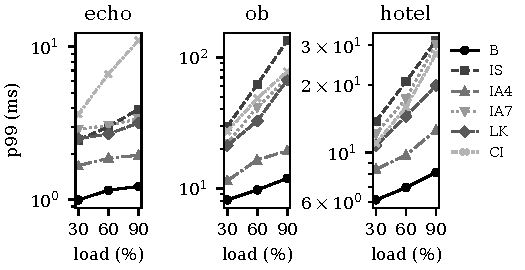
\includegraphics[width=\columnwidth]{figs/p99_carga.pdf}
  \caption{p99 latency vs.\ load level (median of 10 runs; 5 for CI4, run on a
           later day; bands:
           95\% bootstrap confidence interval of the median). Load levels are
           fixed rates, 30/60/90\% of the lowest initial saturation
           estimate (\cref{sec:load}).}
  \label{fig:p99load}
\end{figure}

\begin{table*}[t]
  \centering
  \caption{p99 latency (ms), median of 10 runs (5 for CI4, run on a later day). $^{*}$: different from B
           (Mann--Whitney, Holm-corrected within each column, $p<0.05$).}
  \label{tab:p99}
  \small
  % generated by analysis/20_estatistica.py; do not edit by hand
\begin{tabular}{lrrrrrrrrr}
\toprule
Config. & Echo 30\% & Echo 60\% & Echo 90\% & OB 30\% & OB 60\% & OB 90\% & HR 30\% & HR 60\% & HR 90\% \\
\midrule
B & 1.00 & 1.15 & 1.22 & 8.14 & 9.70 & 11.88 & 6.14 & 6.97 & 8.14 \\
IS & 2.46$^{*}$ & 3.00$^{*}$ & 3.91$^{*}$ & 29.58$^{*}$ & 61.73$^{*}$ & 133.70$^{*}$ & 13.76$^{*}$ & 20.67$^{*}$ & 31.46$^{*}$ \\
IA4 & 1.67$^{*}$ & 1.87$^{*}$ & 1.95$^{*}$ & 11.40$^{*}$ & 16.44$^{*}$ & 19.30$^{*}$ & 8.39$^{*}$ & 9.74$^{*}$ & 12.54$^{*}$ \\
IA7 & 2.88$^{*}$ & 3.07$^{*}$ & 3.38$^{*}$ & 21.95$^{*}$ & 41.51$^{*}$ & 69.31$^{*}$ & 12.11$^{*}$ & 17.35$^{*}$ & 30.35$^{*}$ \\
LK & 2.51$^{*}$ & 2.69$^{*}$ & 3.17$^{*}$ & 21.10$^{*}$ & 32.56$^{*}$ & 66.88$^{*}$ & 10.73$^{*}$ & 14.49$^{*}$ & 19.88$^{*}$ \\
CI & 3.63$^{*}$ & 6.64$^{*}$ & 10.97$^{*}$ & 27.16$^{*}$ & 48.39$^{*}$ & 77.48$^{*}$ & 10.96$^{*}$ & 15.91$^{*}$ & 27.40$^{*}$ \\
CI4 & 3.03$^{*}$ & 2.99$^{*}$ & 2.78$^{*}$ & 11.92$^{*}$ & 14.33$^{*}$ & 18.37$^{*}$ & 7.72$^{*}$ & 8.54$^{*}$ & 10.20$^{*}$ \\
\bottomrule
\end{tabular}
% p99_ms: median of 10 runs (5 for CI4); * = different from B (Mann-Whitney, Holm within each column, p<0.05)

\end{table*}

\paragraph{CPU and memory}
\Cref{fig:resources} breaks CPU down by component, normalized per
1{,}000\,req/s. At 90\% load, among meshes with workload mTLS, Ambient L4 adds
the least CPU (+33\% to +61\% depending on the application), while CI adds the
most on echo and OB (+93\% on OB and
+306\% on echo). The Istio sidecar adds +215\% on echo and +116\% on HR.
On OB at 60\% load, the setting used in the abstract, the extra CPU over
the baseline is 2.6 (IA4), 4.1 (IA7), 4.5 (LK), 6.7 (IS), and 7.0 (CI) cores
per 1{,}000\,req/s. Container CPU misses kernel work done outside any
container, such as WireGuard's encryption in softirq context: CI4's container
CPU is within 7\% of the baseline's at 90\% load and within 13\% at any load. Counting all busy CPU in the four VMs
instead, at the same setting the meshes add 2.0 (CI4), 3.0 (IA4), 4.6 (IA7),
5.2 (LK), 7.5 (IS), and 9.1 (CI) cores per 1{,}000\,req/s, in the same order
as container CPU for the other meshes; in the same-day control, CI4 adds 2.0
and IA4 2.5. Per-request CPU falls with load in every
configuration, most for the L7 proxies (IS's sidecars on OB: 8.1, 6.7, and 4.8
cores per 1{,}000\,req/s at 30, 60, and 90\% load), consistent with more
requests handled per wakeup as queues build; at 90\% load the application
containers under IS and IA7 also use less CPU per request than in the baseline
(3.8 and 4.2 against 5.0), which we have not explained. Relative CPU overheads
are therefore smaller at 90\% than at 60\% load. The dominant component differs by design (OB, 90\% load): the per-pod proxies for the Istio
sidecar and Linkerd (on OB, 4.8 and 3.6 cores per 1{,}000\,req/s), ztunnel
for Ambient L4 (2.1), ztunnel and the waypoint in similar shares for IA7 (1.3
and 1.9), and, for Cilium, the agent and the per-node Envoy in equal parts (2.6
and 3.1). Memory is mostly a fixed cost: the Istio sidecars hold 1.8\,GiB
across the 32 application pods (about 57\,MiB each), against 0.21\,GiB for
Linkerd's proxies (about 7\,MiB each); ztunnel uses about 100\,MiB in total and
the three waypoints 375\,MiB. On the control-plane node, istiod uses 85\,MiB
with sidecars and 155\,MiB in ambient mode, and Linkerd's control plane
140\,MiB. With Istio sidecars, Prometheus also holds about 0.9\,GiB more,
because it scrapes the metrics of every sidecar; we count it as monitoring,
not as mesh cost.

\begin{figure}[t]
  \centering
  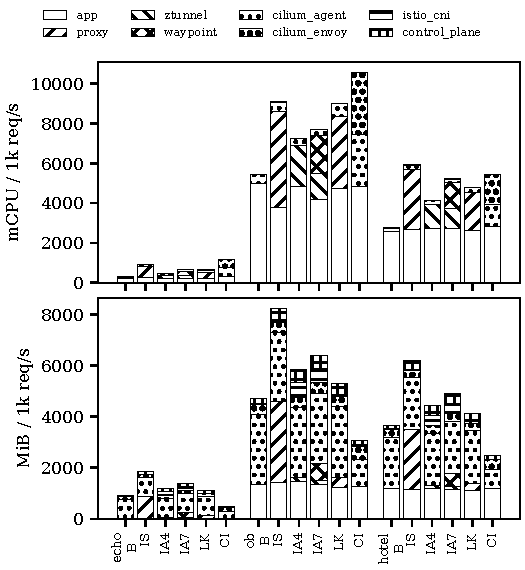
\includegraphics[width=\columnwidth]{figs/recursos.pdf}
  \caption{Container CPU and memory per 1{,}000\,req/s by component, at 90\%
           load (5 runs for CI4, on a later day; its WireGuard work runs in the kernel and
           is not attributed to any container).}
  \label{fig:resources}
\end{figure}

\paragraph{Energy}
\Cref{tab:energy} reports package energy per request, net of the no-mesh idle
power, from a separate run with KVM halt-polling disabled (\cref{sec:design,sec:threats}). Every mesh costs energy, and the ranking mostly follows CPU. At
90\% load, Ambient L4 adds 19--62\% per request (the waypoint is marginally
lower on OB, +16\%), the Istio sidecar 22--129\%,
and Cilium the most, 49--188\%, with its largest overhead on echo. Relative
overheads are lower on OB, where the application itself dominates the energy
per request, and higher at 30\% load, where fixed costs are spread over fewer
requests. With no load, the meshes draw 0.3 (Cilium) to 1.6\,W (Istio sidecar)
above the baseline's 21.0\,W, the sidecar paying for one idle proxy per pod. We did not measure the energy of CI4.

\begin{table}[t]
  \centering
  \caption{Package energy per request (mJ), net of the no-mesh idle power,
           with KVM halt-polling disabled (median of 3 runs).}
  \label{tab:energy}
  \footnotesize
  \setlength{\tabcolsep}{2.5pt}
  % generated by analysis/60_energia.py
\begin{tabular}{lrrrrrr}
\toprule
Config. & Echo 30\% & Echo 90\% & OB 30\% & OB 90\% & HR 30\% & HR 90\% \\
\midrule
B & 4.1 & 2.9 & 48.5 & 36.8 & 19.8 & 16.7 \\
IS & 10.0 & 6.6 & 84.7 & 44.8 & 40.6 & 28.7 \\
IA4 & 6.5 & 4.6 & 67.2 & 43.9 & 30.5 & 23.6 \\
IA7 & 8.1 & 5.7 & 79.3 & 42.8 & 40.1 & 29.1 \\
LK & 8.1 & 5.5 & 78.5 & 49.0 & 35.6 & 26.6 \\
CI & 11.6 & 8.2 & 94.0 & 55.0 & 38.8 & 29.2 \\
\bottomrule
\end{tabular}
% mJ per request, net of the idle power of B, halt_poll_ns = 0

\end{table}

\paragraph{Variability}
Results are stable across repetitions: the coefficient of variation of p99
never exceeds 0.22 (Linkerd on OB at 90\% load). Five of the 540 runs, all on
HR, had error rates between 0.13\% and 0.38\%, and one dropped 37 requests;
all are below the 1\% threshold and are kept.

\section{RQ2: Where Does the Cost Come From?}
\label{sec:rq2}

We profiled every configuration at 60\% load on echo and OB
(\cref{sec:design}) and attribute to the data plane all samples of the proxy
processes (Envoy, \texttt{linkerd2-proxy}, ztunnel, the Cilium agent) plus any
kernel stack that runs WireGuard or an eBPF program. \Cref{fig:perfil}
breaks this CPU down per request and \cref{tab:perfil} summarizes it.

\paragraph{What each data plane spends}
On OB, the baseline spends 0.64\,ms of CPU per request in its data plane (the
Cilium agent and the CNI's eBPF programs, which every configuration also
runs; the increase of a mesh is its total minus this). The Istio sidecar spends 5.5\,ms, of which 61\% is
HTTP/2 framing and header compression (\texttt{nghttp2}): with 11 internal
calls per request, each crossing two sidecars, protocol processing dominates,
as MeshInsight found for an older Envoy~\cite{zhu2023meshinsight}. Ambient L4
spends 2.6\,ms, almost half of it (47\%) in TLS inside ztunnel and no L7
parsing; adding the waypoint (IA7) raises it to 4.2\,ms, split between the
waypoint's HTTP processing (39\%) and ztunnel's TLS (31\%). Linkerd spends
4.6\,ms; because its proxy is distributed without symbols, 46\% of it can only
be attributed to the proxy as a whole, and 13\% is kernel networking. Every
mesh also multiplies kernel crossings: on OB, the data-plane processes (the
proxies and the Cilium agent) make 191 (IS) to 329 (CI) system calls and 58 to
152 context switches per request, against 48 and 31 for the Cilium agent alone
in the baseline.

\paragraph{Why Cilium is the slowest on echo}
On echo, Cilium spends 0.92\,ms of data-plane CPU per request, 9.6$\times$ the
baseline and 1.6$\times$ the Istio sidecar, although the request crosses a
single internal hop. Every request is redirected to the per-node Envoy by the
L7 rule on both nodes, is encrypted by WireGuard (14\% of the total), and makes
the Cilium agent spend almost as much CPU as Envoy itself (36\,s against 39\,s
over the profiling window). It also has the most context switches per request
(27, against 12 for the sidecar). We could not resolve the agent's symbols, so
we located the agent's cost with ablations, run together with a same-day
control of CI (echo, 3 runs each). With Hubble, Cilium's flow observability,
disabled, the agent's CPU at 90\% load falls from 0.96 to 0.36 cores and p99
from 14.4 to 6.7\,ms (8.2 to 4.7\,ms at 60\%): Hubble accounts for 43--54\%
of CI's p99, and every run without it was faster than every run with it. Also
disabling Envoy's access log changes neither. Removing the L7 rule while
keeping WireGuard (CI4) brings p99 down to 1.7\,ms on the same day. The eBPF programs themselves are cheap: with
\texttt{kernel.bpf\_stats\_enabled}, all of Cilium's programs together run
for 40\,\textmu s per echo request and 354\,\textmu s per OB request, 4--5\%
of its data-plane CPU, and the difference to CI4 (19 and 88\,\textmu s) comes
mostly from the program that handles traffic returning from the node's Envoy
(\texttt{cil\_from\_host}). Cilium's overhead therefore comes from redirecting
traffic to the per-node Envoy and from logging every L7 flow to Hubble, not from
its eBPF datapath.

\paragraph{Why the Istio sidecar is the slowest on OB}
On OB, Cilium spends even more CPU per request than the sidecar (7.2 against
5.5\,ms; cAdvisor gives the same order, 7.0 against 6.7 extra cores per
1{,}000\,req/s, \cref{sec:rq1}), yet its p99 is lower (77 against 134\,ms at 90\% load). The
difference is where the work runs. The sidecar's cost follows the frontend,
which issues 10 of the 11 internal calls per request through its own proxy:
that one sidecar uses 1.1--1.3 cores at 90\% load with two worker threads,
while Cilium's per-node Envoys split the L7 work among the nodes that receive
the calls (at most 0.7 cores each). Isolating the frontend on its own node does
not change this, and does not reduce the sidecar's p99 (\cref{sec:rq3}).

\begin{figure}[t]
  \centering
  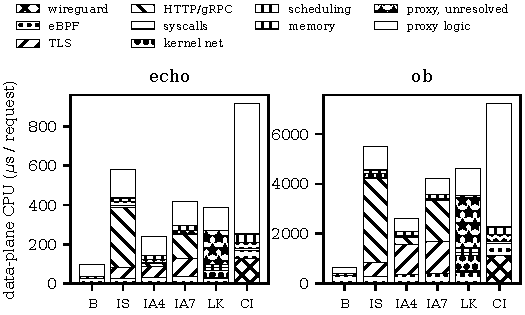
\includegraphics[width=\columnwidth]{figs/perfil.pdf}
  \caption{Data-plane CPU per request by category, at 60\% load (sum of the
           three workers).}
  \label{fig:perfil}
\end{figure}

\begin{table}[t]
  \centering
  \caption{Data-plane CPU per request at 60\% load, share spent in
           cryptography (TLS and WireGuard) and HTTP/gRPC processing, and
           context switches (cs) and system calls (sys) per request of the
           data-plane processes (proxies and the Cilium agent; only the agent
           in B). LK: proxy without symbols, so its TLS and HTTP shares cannot
           be separated.}
  \label{tab:perfil}
  \small
  \setlength{\tabcolsep}{3pt}
  % generated by analysis/50_perfil.py
\begin{tabular}{llrrrrr}
\toprule
App & Config. & CPU ($\mu$s/req) & TLS+WG & HTTP & cs/req & sys/req \\
\midrule
Echo & B & 95 & 0\% & 0\% & 7.6 & 12.5 \\
Echo & IS & 584 & 10\% & 52\% & 12.4 & 36.8 \\
Echo & IA4 & 240 & 24\% & 6\% & 12.7 & 29.9 \\
Echo & IA7 & 418 & 22\% & 30\% & 15.7 & 46.9 \\
Echo & LK & 389 & -- & -- & 14.0 & 30.8 \\
Echo & CI & 916 & 14\% & 0\% & 26.7 & 61.7 \\
OB & B & 641 & 0\% & 0\% & 31.0 & 47.7 \\
OB & IS & 5485 & 11\% & 61\% & 58.1 & 190.6 \\
OB & IA4 & 2591 & 47\% & 10\% & 82.1 & 264.2 \\
OB & IA7 & 4206 & 31\% & 39\% & 68.9 & 302.9 \\
OB & LK & 4624 & -- & -- & 71.4 & 219.5 \\
OB & CI & 7213 & 16\% & 0\% & 151.8 & 329.2 \\
\bottomrule
\end{tabular}

\end{table}

\section{RQ3: Can the Overhead Be Predicted?}
\label{sec:rq3}

\paragraph{Model}
We model the p99 latency added by a mesh as
\begin{equation}
  \Delta L = c_{p}\, P + c_{x}\, X + q\, \frac{\rho_{\text{hot}}}{1-\rho_{\text{hot}}},
  \label{eq:model}
\end{equation}
where $P$ is the number of proxy traversals per request, $X$ the number of
cross-node traversals on the mesh's path, $\rho_{\text{hot}}$ the measured CPU
utilization of the busiest worker, and $c_p$, $c_x$, and $q$ are fitted per
mesh. $P$ and $X$ come from the call graph measured with Istio telemetry and
from the pod placement: echo makes 1 internal call per request (across
nodes), OB 11 (10.4 across nodes), and HR 3.8 (1.0 across nodes). A sidecar
mesh adds two traversals per call; ztunnel one per node the call touches; the
waypoint one more per call, plus up to two cross-node hops between client,
waypoint, and server; Cilium's node Envoy one per call, at the destination's
node, where the ingress L7 rule applies (none in CI4); and every mesh except
CI4 one at the entry service (on echo, CI's two Envoy traversals are the entry
and the call). We fit by non-negative least
squares on echo and OB and predict HR, which is held out, and the placement
experiment below, which no fit has seen. Each fit has three parameters and six
points (two applications, three loads), and $\rho_{\text{hot}}$ is measured at
the target load, so the model explains rather than forecasts. As a variant,
we replace
$\rho_{\text{hot}}$ with $\rho_{\text{proxy}}$, the utilization of the busiest
proxy instance: its CPU divided by its worker threads (two for Istio sidecars,
waypoints, and ztunnel; one for \texttt{linkerd2-proxy}; four, the node's
vCPUs, for Cilium's Envoy).

\paragraph{Results}
\Cref{tab:model} shows the fitted costs and the prediction errors. The
clearest positive result is for the per-pod sidecars: with queueing at the
busiest proxy instance instead of the busiest node, the held-out error on HR
falls from 82\% to 19\% for Linkerd and from 135\% to 52\% for the Istio
sidecar. The model also works for the two L4 data planes: it predicts HR's p99 within 11\% for Ambient
L4, with 120\,\textmu s per ztunnel traversal, and within 13\% for CI4, with
277\,\textmu s per cross-node traversal, the cost of WireGuard. The busiest
proxy instance of the per-pod meshes is the frontend's sidecar; Linkerd's,
single-threaded, reaches 0.91 of its thread on OB at 90\% load. The proxy
term does not help the shared proxies (86\% for IA7, 144\% for CI), and with
node utilization the L7 errors range from 82\% (Linkerd) to 140\% (CI); for
the Istio sidecar and the waypoint that fit assigns the whole overhead to the
queueing term ($c_p = 0$). The cross-node term never helps ($c_x = 0$) except
for CI4. With node utilization, the model overpredicts the L7 meshes on HR by
about 2$\times$: at 90\% load HR's busiest worker is 55--68\% utilized
under the L7 meshes, close to OB's 53--76\%, yet HR's p99 increase is 2.6--5.2
times smaller, so node utilization is not what sets their tail.

\begin{table}[t]
  \centering
  \caption{Model of the p99 increase (\cref{eq:model}), fitted on echo and OB,
           with the queueing term on the busiest node or on the busiest
           proxy instance. Median relative errors on HR (held out), on the
           placement cells (\cref{tab:placement}), and of the bottleneck law
           $X_{\max} \approx \lambda/\rho_{\text{hot}}$ (median over OB
           and HR). $c_p$, $c_x$, $q$: node variant.}
  \label{tab:model}
  \footnotesize
  \setlength{\tabcolsep}{2.5pt}
  % generated by analysis/40_modelo.py
\begin{tabular}{lrrrrrr}
\toprule
Config. & $P_\mathrm{hotel}$ & $c$ ($\mu$s) & err. mean & $c_{p99}$ ($\mu$s) & err. p99 & LOLO p99 \\
\midrule
IS & 8.6 & 0 & 199\% & 0 & 135\% & 111\% \\
IA4 & 5.8 & 72 & 22\% & 120 & 11\% & 27\% \\
IA7 & 9.6 & 0 & 237\% & 0 & 140\% & 75\% \\
LK & 8.6 & 112 & 82\% & 55 & 82\% & 39\% \\
CI & 5.8 & 295 & 145\% & 458 & 131\% & 60\% \\
\bottomrule
\end{tabular}

\end{table}

\paragraph{Placement}
To test whether the busiest node sets the tail, we repeated OB at the 60\% and
90\% rates (5 runs each) with two other placements, together with a same-day
control, IA7 in the original placement, which reproduced the main run at 90\% load (70.5
against 69.3\,ms; 36.7 against 41.5\,ms at 60\%). In \emph{fe-alone}, the frontend, which issues
10 of the 11 internal calls, runs alone on its worker and the other ten
services alternate on the other two (B, IS, IA7). In \emph{wp-moved}, IA7's
waypoint moves to the worker that was least loaded in the original placement
(it becomes the busiest). \Cref{tab:placement} shows that
the changes are only partly consistent with a node-level explanation. Under
fe-alone, IA7's busiest worker rose from 51\% to 72\% and its p99 from 71 to
106\,ms, as that explanation predicts. But isolating the frontend lowered
IS's busiest worker from 76\% to 60\% at 90\% load with little change in
p99 (134 to 128\,ms against the main run); a same-day control a week later
confirms it, with the busiest worker going from 82\% to 60\% and p99 falling
by only 8\% (211 to 195\,ms; 10\% at 60\% load), and moving the waypoint to the
least-loaded worker nearly doubled IA7's p99 (71 to 125\,ms) with a small
change in node load (51\% to 58\%). Cross-node traversals change by at most 6\% between
placements, so they do not explain these differences either. What placement
does not change is the load on the single busiest proxy, which in every L7
mesh handles most of OB's calls: the frontend's sidecar (1.1--1.3 cores with
two worker threads under IS, 0.9 with one under Linkerd) and the OB waypoint
(1.0--1.1 cores in every placement). For IS this explains fe-alone better than
the node does (placement error 22\% against 40\%), but it cannot explain
wp-moved, where the waypoint's utilization is unchanged (0.52) and p99 nearly
doubles. The waypoint's new node also receives all external traffic (the
NodePort entry) and runs the most-called service; we did not separate these
effects.

\begin{table}[t]
  \centering
  \caption{OB placement experiment (5 runs per cell; same-day control for
           IA7; 3 runs for the IS pair from the same-day control a week
           later). p99 in ms at the 60\% and 90\% rates; $\rho_{\text{hot}}$:
           busiest worker at 90\%; $X$: cross-node traversals per request,
           including the entry hop.}
  \label{tab:placement}
  \footnotesize
  \setlength{\tabcolsep}{3pt}
  \begin{tabular}{@{}llrrrr@{}}
    \toprule
    Config. & Placement & p99 60\% & p99 90\% & $\rho_{\text{hot}}$ & $X$ \\
    \midrule
    B   & original (main run)      & 9.7  & 11.9  & .43 & 11.4 \\
    B   & fe-alone                 & 9.6  & 11.9  & .44 & 12.0 \\
    IS  & original (main run)      & 61.7 & 133.7 & .76 & 11.4 \\
    IS  & fe-alone                 & 59.8 & 128.4 & .60 & 12.0 \\
    IS  & original (later day)     & 95.1 & 211.3 & .82 & 11.4 \\
    IS  & fe-alone (later day)     & 85.2 & 194.9 & .60 & 12.0 \\
    IA7 & original (control)       & 36.7 & 70.5  & .51 & 17.6 \\
    IA7 & fe-alone                 & 49.4 & 106.3 & .72 & 16.6 \\
    IA7 & wp-moved                 & 51.4 & 124.7 & .58 & 18.0 \\
    \bottomrule
  \end{tabular}
\end{table}

\paragraph{Throughput}
A simpler bottleneck law predicts saturation well: dividing the 90\% rate by
the busiest worker's utilization, $X_{\max} \approx \lambda/\rho_{\text{hot}}$,
matches the measured maximum throughput (\cref{tab:sat}) on OB and HR within
19\% for every configuration (median 6\%). It overestimates echo by 37--53\%
for all configurations but the two L4 data planes (6\% and 15\%), because
echo saturates in a single process, the Fortio relay, before its node does.

We therefore read RQ3 as a partial answer. Per-traversal costs predict the
overhead of L4 data planes, and node utilization predicts throughput on OB and HR. For L7
data planes, neither per-hop costs, cross-node hops, nor node utilization
predict the tail; the utilization of the busiest proxy instance does better for
per-pod sidecars, but not for shared proxies or for moving the waypoint.

\section{RQ4: Which Mesh Should I Use?}
\label{sec:rq4}

\Cref{tab:guide} condenses our results into a decision guide; pairwise
comparisons cited there are significant (Mann--Whitney, Holm-corrected within
each application and load, $p<0.05$) unless stated otherwise. Two observations
cut across it. First, the cheapest mesh is the one that does the least per
request. Among the meshes that authenticate workloads, Ambient L4 avoids L7
parsing entirely and is the cheapest on every metric we measured (the one
exception, energy per request on OB at 90\% load, is within 3\% of the
waypoint). Cilium without L7 rules (CI4) is cheaper still in CPU, counting the
kernel time of its WireGuard, which container CPU does not show, and in p99 on
HR, but it authenticates nodes, not workloads, and leaves same-node traffic
unencrypted.
Second, for L7 data planes, the tail is not predicted by per-hop cost or by
node utilization (\cref{sec:rq3}); in the one case where moving pods
relieved the busiest node (IS, from 82\% to 60\% in a same-day control), p99
fell by only 8--10\%. For per-pod sidecars, the load on the busiest proxy
instance, the sidecar of the fan-out service, predicts it better. Capacity
planning for L7 meshes should therefore measure the tail under the intended
placement rather than infer it from node utilization.

\begin{table}[t]
  \centering
  \caption{Decision guide. Evidence at 90\% load unless stated otherwise.}
  \label{tab:guide}
  \footnotesize
  \setlength{\tabcolsep}{3pt}
  \begin{tabular}{@{}>{\raggedright\arraybackslash}p{0.25\columnwidth}>{\raggedright\arraybackslash}p{0.17\columnwidth}>{\raggedright\arraybackslash}p{0.52\columnwidth}@{}}
    \toprule
    Need & Choose & Evidence \\
    \midrule
    Workload mTLS, L4 policy only & IA4 & lowest p99 increase among meshes with
      workload mTLS (+54 to +62\%), 78--82\% of no-mesh throughput, least CPU;
      no L7 parsing (\cref{sec:rq2}) \\
    Node-to-node encryption suffices & CI4 & p99 +25\% (HR, below IA4), +55\%
      (OB, like IA4), echo inconclusive (1.7--3.0\,ms across days); 82--87\% of no-mesh throughput; fewest
      extra cores; no workload identity, same-node traffic in clear \\
    L7 policy, deep call graphs & LK & p99 on OB: +463\% (LK) and +483\%
      (IA7; not significantly different) vs.\ +1025\% (IS); on HR, LK +144\%,
      IA7 +273\% (not different from IS, +286\%) \\
    L7 on a high fan-out service & LK or IA7; test placement & node load
      explains the tail only partly: isolating the frontend lowered IS's p99 by
      8--10\% (same day) while its node went from 82\% to 60\%; moving the waypoint to the least-loaded node raised IA7's from 71 to
      125\,ms \\
    Smallest memory footprint & IA4 or LK & ztunnel 100\,MiB in total; Linkerd
      7\,MiB per pod vs.\ 57\,MiB for Istio sidecars \\
    Already on Cilium & CI4, or scoped L7 rules with Hubble off & the L7
      redirect and Hubble, not eBPF (4--5\% of data-plane CPU), make CI the
      most expensive mesh; Hubble off cuts echo p99 by 43--54\% \\
    \bottomrule
  \end{tabular}
\end{table}

\section{Threats to Validity}
\label{sec:threats}

\paragraph{Single host}
All VMs share one host, memory bus, and last-level cache. We mitigate this by
pinning every vCPU to a dedicated physical thread, but absolute numbers will
differ on physical clusters: our reproduction of MeshInsight matches its CPU
overheads but not its latency overheads (\cref{sec:validation}). Relative results are stable across deployments: a second,
independent deployment of every configuration reproduced the p99 ranking
(\cref{sec:rq1}).

\paragraph{Energy under virtualization}
RAPL measures the whole package, including the hypervisor. In our main
experiment, KVM halt-polling was enabled (200\,\textmu s): an idle vCPU spins
on the host before sleeping, which draws power without showing up as busy CPU
inside the guest. Disabling it cut package power by 10--23\% at every load and
raised the relative energy cost of every mesh, because the baseline, with the
most short idle periods, had been inflated the most; on OB at 90\% load the
Istio sidecar went from 8\% below the baseline to 22\% above it. We therefore
report energy from a run with halt-polling disabled and recommend
\texttt{halt\_poll\_ns=0} for RAPL-based energy studies in virtual machines.
Even then, the Istio sidecar draws about 1.6\,W less than a linear fit of power
against in-guest busy cores predicts, so in-guest CPU is only an approximate
proxy for host power.

\paragraph{Ordering}
Runs are randomized within each configuration, but configurations ran in
blocks. An interleaved control experiment (B and IS alternated in blocks, with
halt-polling enabled) reproduced the power difference observed in the main run
at the same temperatures, which makes time of day and temperature unlikely
causes; the smaller residual reported under Energy under virtualization persists
with halt-polling disabled.

\paragraph{Encryption scope}
Cilium's WireGuard encrypts only traffic between nodes, so the same-node calls
in our placement (2.8 of HR's 3.8 calls per request) are not encrypted under
CI and CI4, while every other mesh encrypts them. This favors both on HR, and
is part of why CI4 has the lowest overhead there.

\paragraph{Follow-up runs}
CI4 and the placement experiment ran a few days after the main run, and the
Hubble ablation, with a CI control and a repeat of CI4 on echo, a week later,
each after a host reboot, with the
same host settings and rates but fewer repetitions (5, 5, and 3). Same-day
controls bound the effect of the day: IA7 on OB in the original placement
reproduced the main run within 2\% at 90\% load (12\% faster at 60\%), and
the baseline on OB in the fe-alone placement within 2\%, but CI on echo was
24--31\% slower than in the main run and CI4 on echo differed by up to 41\%
between the two days. A third control, a week after the main run, repeated B,
IA4, CI4, and IS on OB and HR and IS with fe-alone on the same day: the
baseline was 5--19\% slower than in the main run and IS on OB up to 58\%
slower, so absolute values move between days more than rankings do, and the
CI4 and placement comparisons we state hold within that day. We therefore compare the
Cilium ablations only within a day and treat cross-day differences on echo of
that size as inconclusive. We did not measure CI4's energy, and placement was
varied only for OB.

\paragraph{Versions and defaults}
Meshes evolve quickly; we pin versions and use default proxy settings, which
may not match tuned production deployments. Default proxy limits did not bind:
the busiest sidecar stayed below its 2-CPU limit (\cref{sec:testbed}).
Cilium shares one CNI configuration with the other meshes, with socket-level
load balancing limited to the host namespace (required by Istio and Linkerd),
and CI keeps Hubble and the Envoy access logs on, as by default; a Cilium-only
deployment could avoid both. Hubble alone accounts for 43--54\% of CI's p99 on
echo (\cref{sec:rq2}).

\paragraph{Applications}
Two benchmark applications and a microbenchmark cannot represent every call
graph; Hotel Reservation keeps most of its calls on the same node under our
placement, which favors node-level proxies.

\section{Conclusion}
\label{sec:conclusion}

We compared seven service-mesh configurations on the same testbed, with open-loop
load and the same absolute request rates for all of them. Among the meshes that
authenticate workloads, Istio Ambient in L4 mode is the cheapest on every
metric except energy on OB at 90\% load (within 3\% of the waypoint): it keeps 78--82\% of the no-mesh throughput and adds 54--62\% to p99 at
90\% load, while the L7 data planes add 144--1025\%. Cilium without L7 rules uses
less CPU and sustains as much or more throughput, with a lower or similar tail on the
two microservice applications, at the price of node-level rather than
workload-level security. Profiling shows where the difference comes
from: HTTP/2 processing for the Istio sidecar, TLS for ztunnel, and, for Cilium,
the redirect to the per-node Envoy and Hubble flow logging rather than eBPF.
Per-hop costs predict the overhead of L4 data planes and node utilization
predicts the throughput of the microservice applications, but neither predicts
the tail of L7 data planes. The utilization of the busiest proxy instance
predicts it better for per-pod sidecars (held-out error 19\% for Linkerd and
52\% for the Istio sidecar, against 82\% and 135\% with node utilization), and
relieving the busiest node lowered the sidecar's tail by only 8--10\%. We release the testbed and
data so that these results can be reproduced and extended.


\bibliographystyle{IEEEtran}
\bibliography{refs}

\end{document}
